\section{Überblick}\label{sec:analyse}

Abbildung \ref{fig:results-evaluation-metrics-comparison} zeigt für jedes der untersuchten Modelle die durchschnittlichen Metrik-Werte über alle fünf Wiederholungen hinweg inklusive Standardabweichung. Für einen besseren Vergleich sind die proprietären Modelle rot, die kleineren Modelle orange und die größeren Modelle blau dargestellt. Diese Einteilung entspricht der in Kapitel \ref{ch:modellauswahl} beschriebenen Kategorisierung. Die Diagramme aus diesem Kapitel stammen nicht direkt aus dem Evaluationsframework, sondern wurden mit den zusammengeführten Ergebnissen aller Experimente erstellt, damit alle Modelle auf einen Blick verglichen werden können. Im Folgenden wird zuerst ein Überblick über die Ergebnisse gegeben, bevor im Anschluss eine detaillierte Analyse erfolgt.

\begin{figure}[htbp]
    \centering
    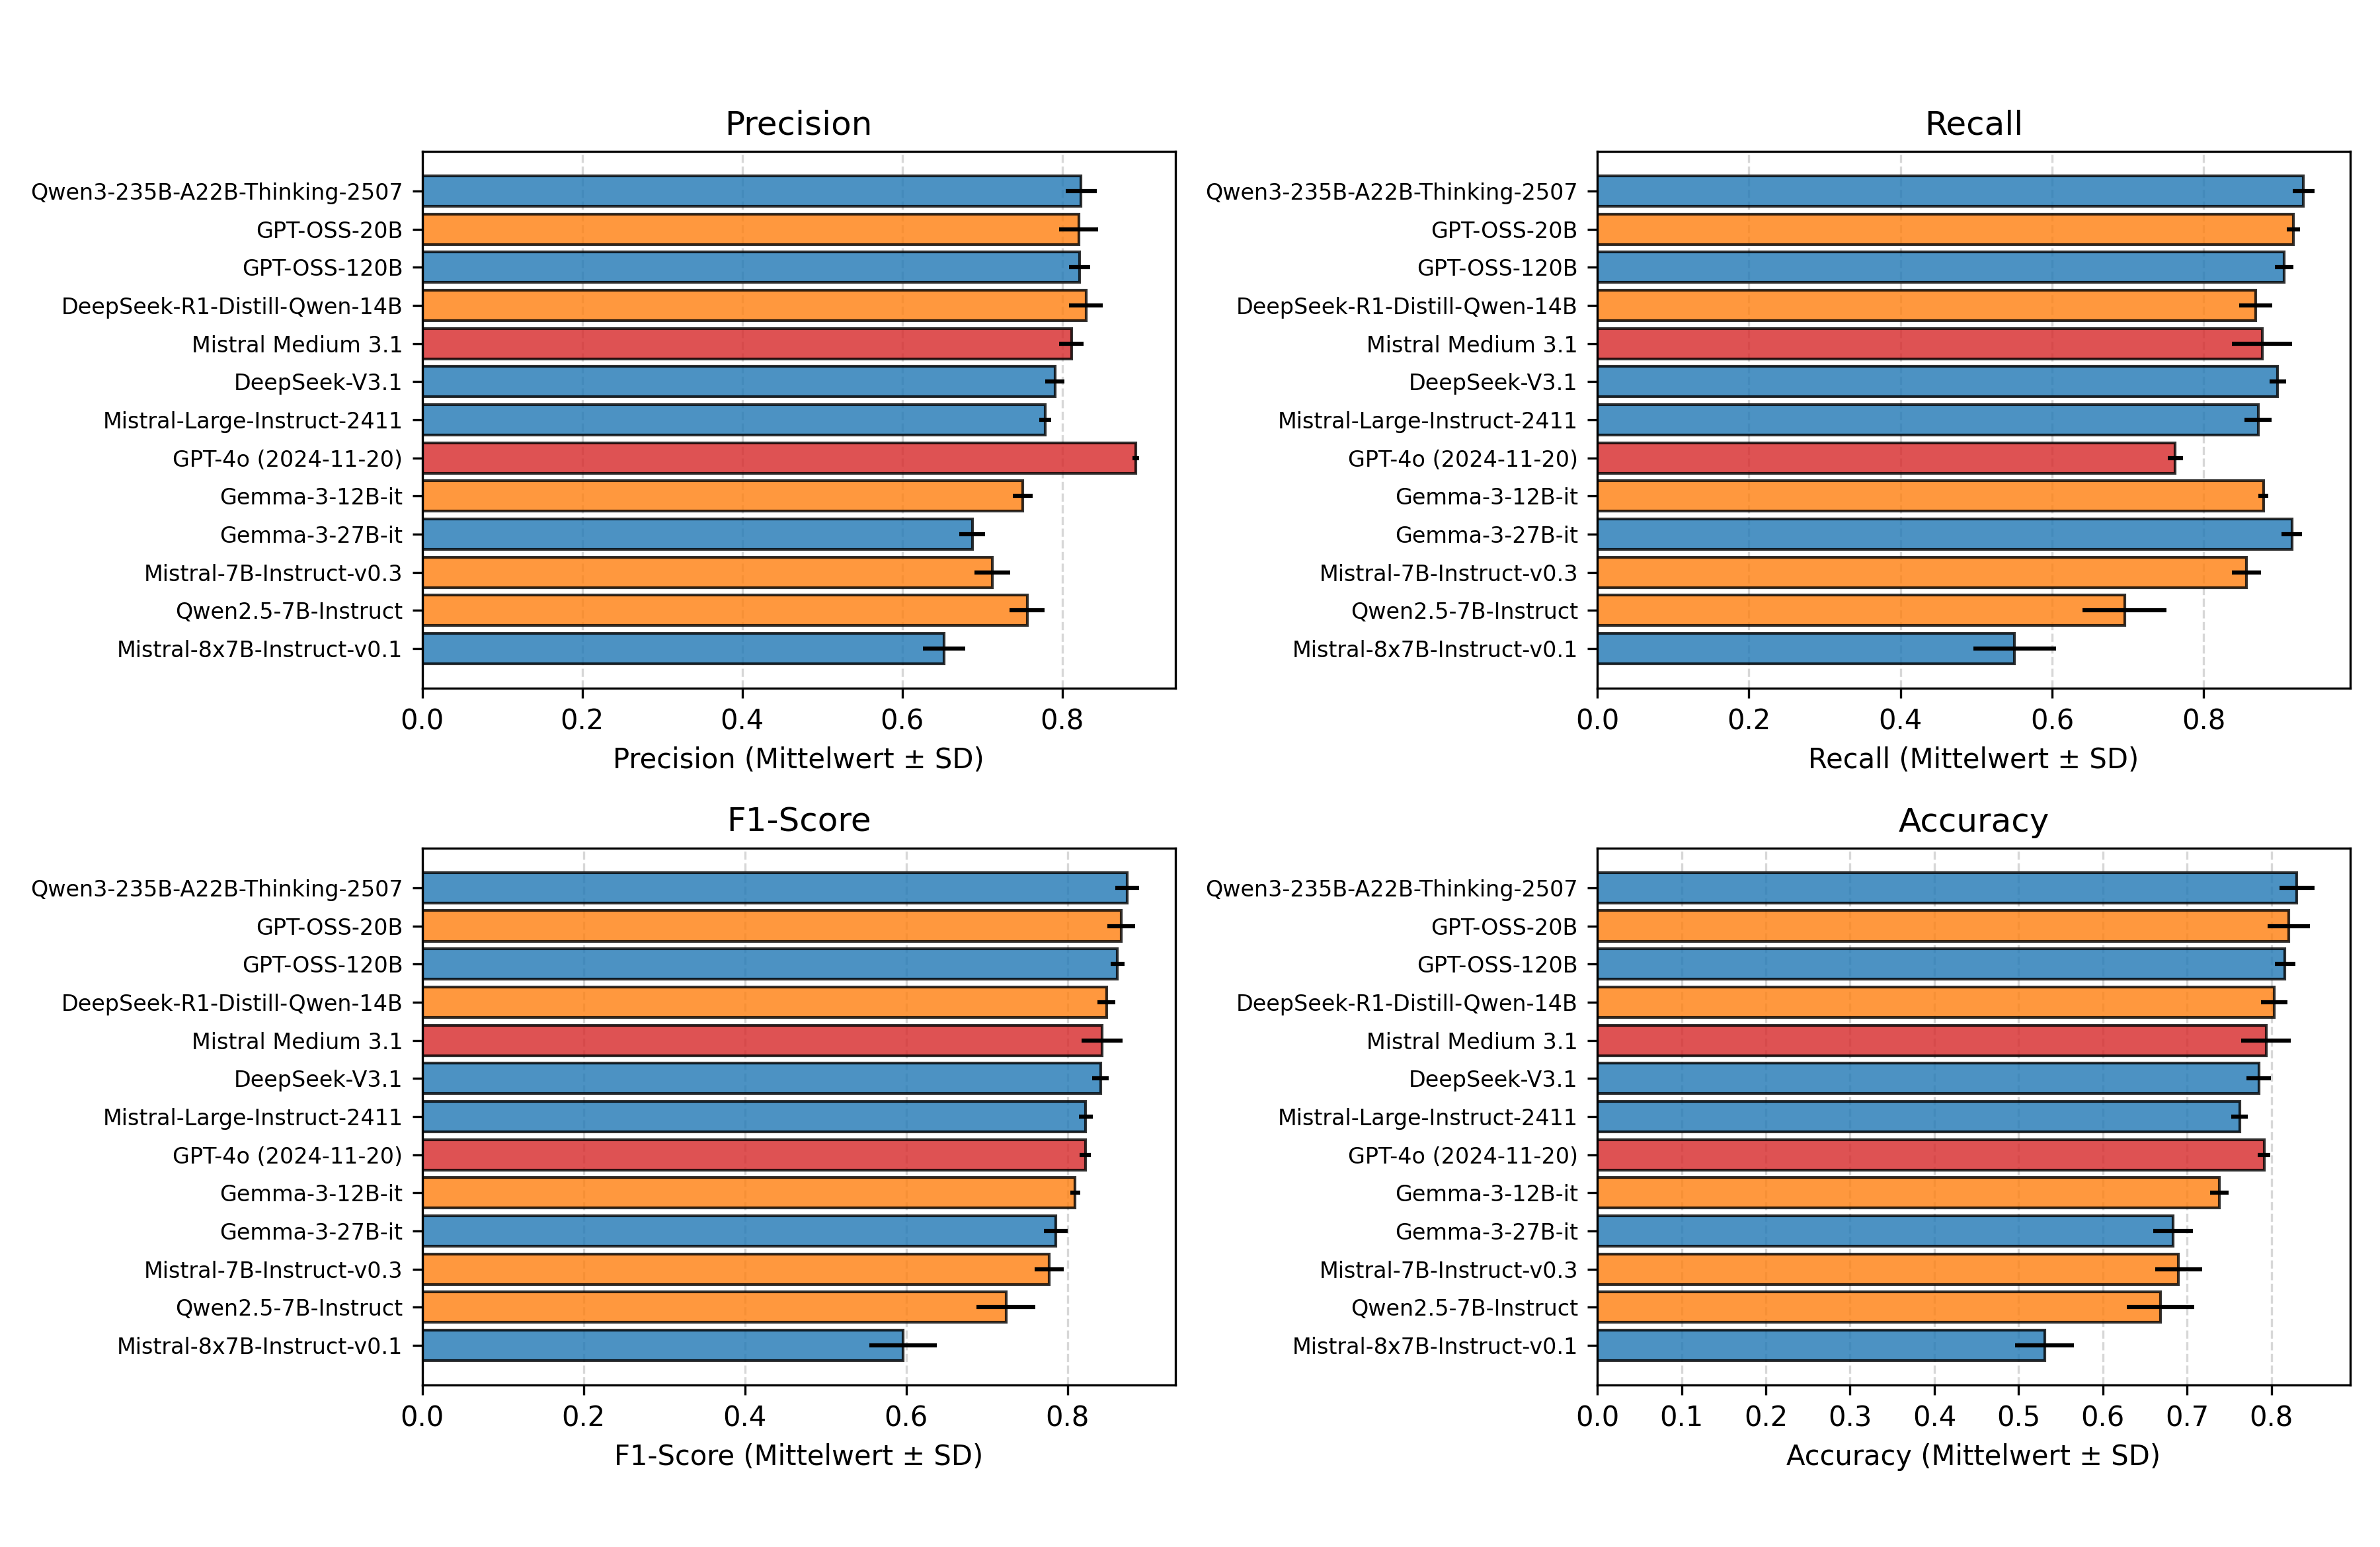
\includegraphics[width=\textwidth,trim=20 40 20 10]{images/results/evaluation_metrics_comparison}
    \caption{Durchschnittliche Metrik-Werte der untersuchten Modelle über alle Wiederholungen hinweg inklusive Standardabweichung.}
    \label{fig:results-evaluation-metrics-comparison}
\end{figure}

Positiv aufgefallen ist, dass neun von dreizehn Modellen das Qualitätsziel eines F1-Scores von $\geq 0{,}80$ erreichen konnten - darunter auch kleine Modelle. Dennoch übertreffen die großen Modell die Kleinen vor allem im F1-Score, was auf eine bessere Balance zwischen Präzision und Recall hindeutet. Über alle Metriken hinweg sind \texttt{Qwen3-235B-A22B-Thinking-2507}, \texttt{GPT-OSS-120B} und \texttt{GPT-OSS-20B} ganz vorne mit dabei. Auffällig ist das schwache Abschneiden des europäischen \texttt{Mistral-8x7B-Instruct-v0.1}-Modells, das sowohl in Precision, als auch Recall weit zurückfällt und als einziges Modell einen F1-Score von $\le 0{,}60$ erreicht.

Die Abbildung \ref{fig:results-evaluation-metrics-comparison} macht deutlich, dass einige Modelle – etwa \texttt{GPT-4o} oder\linebreak\texttt{Qwen-2.5-7B-Instruct} – hohe Präzisionswerte aufweisen, aber im Recall zurückliegen. Anders sieht es bei \texttt{Gemma-3-27B-it} aus, das einen sehr guten Recall erreicht, aber bei der Präzision auf dem vorletzten Platz liegt. Modelle wie \texttt{Qwen3-235B-A22B} und \texttt{GPT-OSS-20B} erreichen einen ausgezeichneten Recall bei gleichzeitig hoher Präzision.

\begin{figure}[htbp]
    \centering
    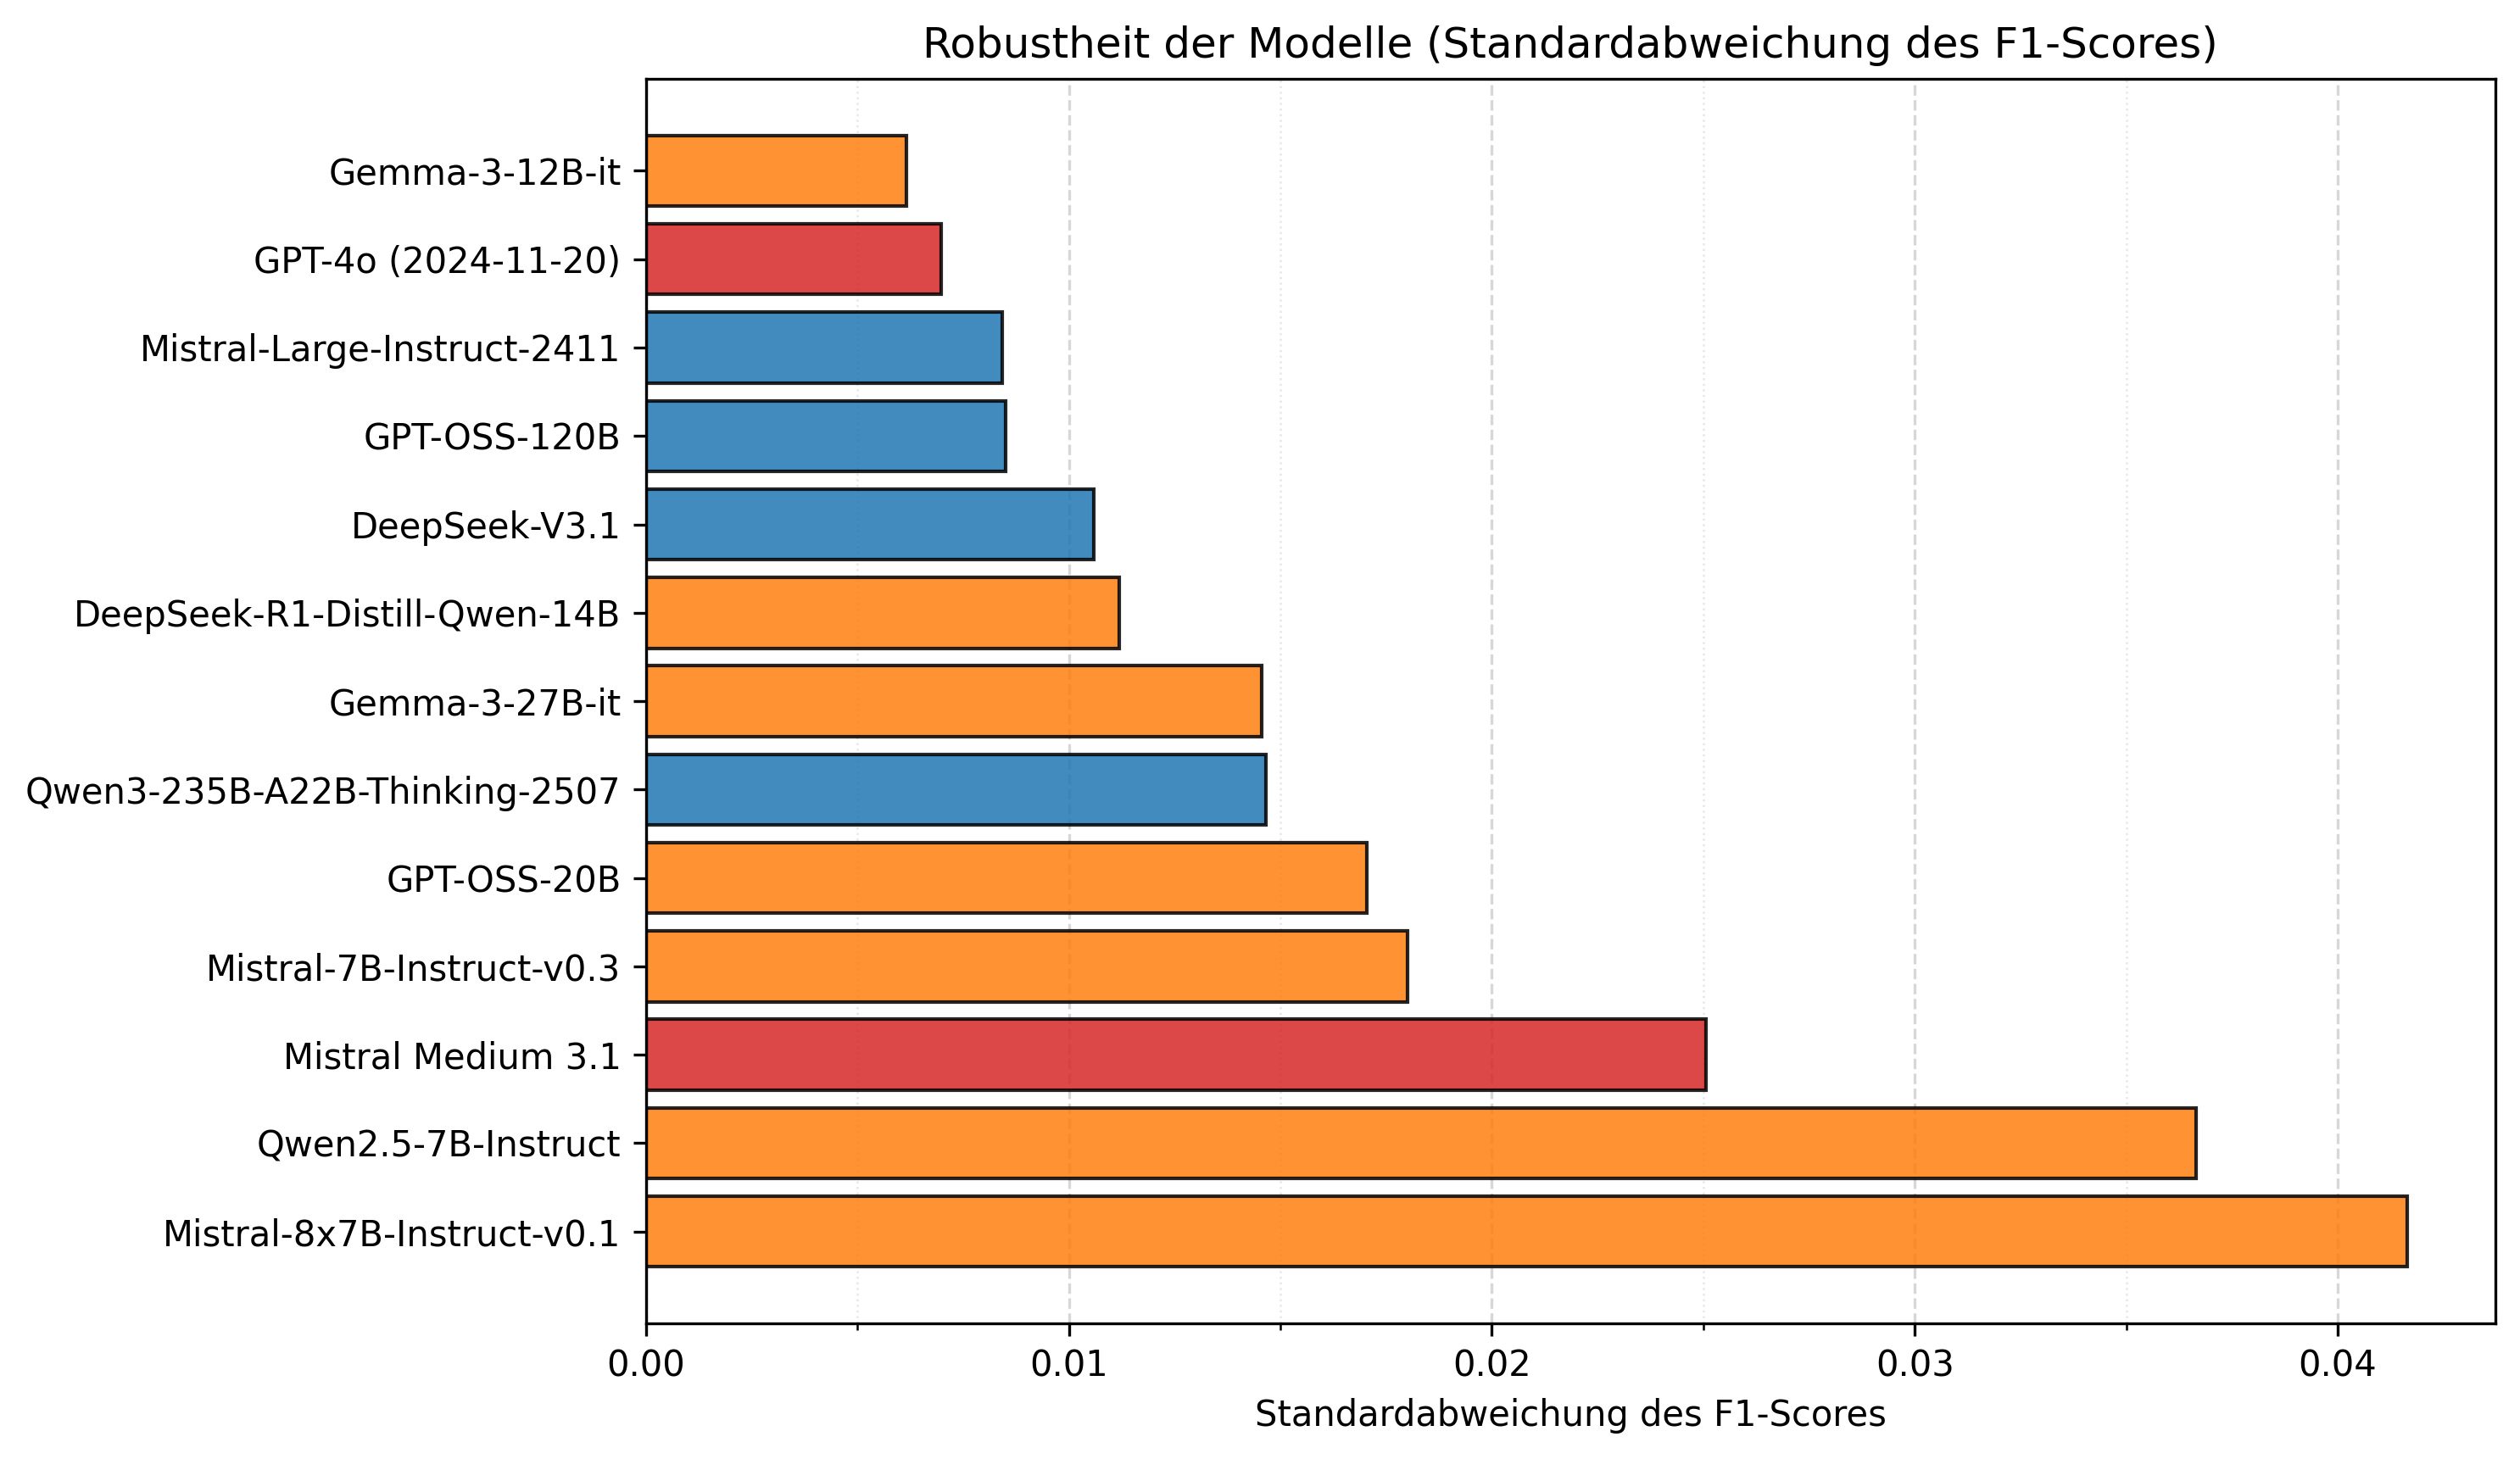
\includegraphics[width=\textwidth]{images/results/evaluation_robustness_f1_std}
    \caption{Robustheit der Modelle gemessen an der Standardabweichung des F1-Scores über alle Wiederholungen hinweg.}
    \label{fig:results-evaluation-robustness-f1-std}
\end{figure}

Abbildung \ref{fig:results-evaluation-robustness-f1-std} zeigt die Robustheit der Modelle gemessen an der Standardabweichung des F1-Scores über alle Wiederholungen hinweg. Hier zeigt sich eine große Varianz: Während einige Modelle wie \texttt{Gemma-3-12B.it} und \texttt{Mistral-Large-Instruct-2411} eine sehr geringe Standardabweichung von $\le 0{,}01$ aufweisen, zeigen andere Modelle wie \texttt{Mistral-8x7B-Instruct-v0.1} und \texttt{Qwen2.5-7B-Instruct} eine hohe Varianz von $\ge 0{,}03$ bis $\ge 0{,}04$ im F1-Score. Dies deutet darauf hin, dass die Leistung dieser Modelle stark von der Wahl des Seeds abhängen und ihre Leistung weniger stabil ist.

Neben den Diagrammen \ref{fig:results-evaluation-metrics-comparison} und \ref{fig:results-evaluation-robustness-f1-std} liefert \autoref{tab:metrics-overview} eine tabellarische
Übersicht der konkreten durchschnittlichen Metrik-Werte inklusive Standardabweichungen für alle Modelle über alle fünf Wiederholungen hinweg. Diese Werte werden genutzt um im Folgenden die Leistungen der Modelle detailliert zu analysieren.

Die proprietären Modelle \texttt{GPT-4o} und \texttt{Mistral Medium 3.1} erreichen mit $0{,}822$ bzw. $0{,}843$ im Vergleichsfeld einen mittleren F1-Score. \texttt{Mistral Medium 3.1} liegt mit
einem F1-Wert von $0{,}843$ leicht über \texttt{GPT-4o} und weist zugleich
einen höheren Recall von $0{,}877$ auf. \textttt{GPT-4o} fällt vor allem durch eine sehr hohe Precision von $0{,}892$ auf, die jedoch einem vergleichsweise niedrigem Recall von $0{,}762$ gegenübersteht. Dies deutet darauf hin, dass \texttt{GPT-4o} eher konservativ kritische Aktivitäten klassifiziert und somit weniger \acp{FP}, aber auch mehr \acp{FN} produziert. Dies
macht das Modell geeignet für strikte Sicherheitsanforderungen, jedoch
weniger für ein Vorscreening, wie es in dieser Arbeit angestrebt wird.

\begin{table}[htbp]
    \centering
    \caption{Aggregierte Mittelwerte und Standardabweichungen der Evaluationsmetriken über alle fünf Wiederholungen hinweg.}
    \label{tab:metrics-overview}
    \begin{adjustbox}{width=\textwidth}
        \begin{tabular}{l r r r r}
            \toprule
            Modell & Precision & Recall & F1-Score & Accuracy \\
            \midrule
            DeepSeek-V3.1 & 0.791 $\pm$ 0.012 & 0.897 $\pm$ 0.011 & 0.841 $\pm$ 0.011 & 0.785 $\pm$ 0.015 \\
            DeepSeek-R1-Distill-Qwen-14B & 0.829 $\pm$ 0.021 & 0.868 $\pm$ 0.022 & 0.848 $\pm$ 0.011 & 0.803 $\pm$ 0.016 \\
            Gemma-3-12B-it & 0.751 $\pm$ 0.013 & 0.879 $\pm$ 0.006 & 0.810 $\pm$ 0.006 & 0.738 $\pm$ 0.011 \\
            Gemma-3-27B-it & 0.687 $\pm$ 0.016 & 0.916 $\pm$ 0.014 & 0.785 $\pm$ 0.015 & 0.683 $\pm$ 0.023 \\
            Mistral-7B-Instruct-v0.3 & 0.712 $\pm$ 0.022 & 0.856 $\pm$ 0.019 & 0.777 $\pm$ 0.018 & 0.690 $\pm$ 0.028 \\
            Mistral-8x7B-Instruct-v0.1 & 0.652 $\pm$ 0.027 & 0.550 $\pm$ 0.054 & 0.596 $\pm$ 0.042 & 0.531 $\pm$ 0.035 \\
            Mistral-Large-Instruct-2411 & 0.779 $\pm$ 0.008 & 0.872 $\pm$ 0.018 & 0.823 $\pm$ 0.008 & 0.762 $\pm$ 0.010 \\
            Mistral Medium 3.1 & 0.811 $\pm$ 0.015 & 0.877 $\pm$ 0.040 & 0.843 $\pm$ 0.025 & 0.794 $\pm$ 0.029 \\
            GPT-OSS-20B & 0.820 $\pm$ 0.024 & 0.918 $\pm$ 0.009 & 0.866 $\pm$ 0.017 & 0.821 $\pm$ 0.025 \\
            GPT-OSS-120B & 0.822 $\pm$ 0.013 & 0.906 $\pm$ 0.012 & 0.862 $\pm$ 0.009 & 0.816 $\pm$ 0.012 \\
            GPT-4o & 0.892 $\pm$ 0.004 & 0.762 $\pm$ 0.010 & 0.822 $\pm$ 0.007 & 0.791 $\pm$ 0.007 \\
            Qwen2.5-7B-Instruct & 0.756 $\pm$ 0.022 & 0.696 $\pm$ 0.055 & 0.724 $\pm$ 0.037 & 0.668 $\pm$ 0.040 \\
            Qwen3-235B-A22B-Thinking-2507 & 0.824 $\pm$ 0.019 & 0.932 $\pm$ 0.014 & 0.874 $\pm$ 0.015 & 0.830 $\pm$ 0.021 \\
            \bottomrule
        \end{tabular}
    \end{adjustbox}
\end{table}

Die Mehrzahl der großen Modelle steht in den meisten Metriken deutlich vor den kleineren Modellen. Ein bemerkenswerter Befund ist jedoch die starke Leistung von \texttt{GPT-OSS-20B}, das mit Blick auf die F1-, Recall- und Accuracy-Werten von $0{,}866$, $0{,}918$ bzw. $0{,}821$ fast mit den besten Modellen mithalten kann und dort sogar besser abschneidet als das größere \texttt{GPT-OSS-120B}. Nur in der Precision liegt \texttt{GPT-OSS-120B} mit $0{,}821$ knapp vor \texttt{GPT-OSS-20B}. Allerdings deuten die Standardabweichungen auf eine geringere Stabilität von \texttt{GPT-OSS-20B} hin. Ein weiteres starkes kelines Open-Source-Modell ist \texttt{DeepSeek-R1-Distill-Qwen-14B}, das in F1-Score und Accuracy die
beiden proprietären Modelle übertrifft und in der Precision sogar über \texttt{Qwen3-235B-A22B-Thinking-2507} und die \texttt{GPT-OSS}-Modelle hinausgeht.

Die Ergebnisse unterstreichen, dass \texttt{Qwen3-235B-A22B-Thinking-2507}, \texttt{Gemma-3-27B-it} und \texttt{GPT-OSS-20B} mit $\geq 0{,}91$ die höchsten Recall Werte erzielen. Dies bedeutet, dass diese Modelle die meisten kritischen Aktivitäten korrekt identifizieren und somit das Risiko von \acp{FN} minimieren. Besonders hervorzuheben ist \texttt{Qwen3-235B-A22B-Thinking-2507}, das mit einem Recall von $0{,}932$ und einer Precision von $0{,}824$ eine ausgezeichnete Balance zwischen Sensitivität und Genauigkeit bietet. Mit Abstand am schwächsten im Recall schneiden \texttt{Mistral-8x7B-Instruct-v0.1} und \texttt{Qwen2.5-7B-Instruct} ab, die mit $0{,}550$ bzw. $0{,}696$ weit hinter den anderen Modellen zurückbleiben.

\texttt{Mistral-8x7B-Instruct-v0.1} schnitt insgesamt am schlechtesten ab. Sowohl die Precision von $0{,}652$ als auch der Recall von $0{,}55$ und die Accuracy von $0{,}531$ sind klar unter den Werten der anderen Modelle. Besonders bemerkenswert ist, dass das kleinere \texttt{Mistral-7B-Instruct-v0.3} – mit achtmal weniger Parametern – deutlich bessere Ergebnisse erzielt. Auch gegenüber dem ähnlich großen \texttt{Qwen2.5-7B-Instruct} ist es im F1-Score und in der Accuracy leicht voraus und im Recall mit einer Differenz von $0{,}106$ schneidet \texttt{Mistral-7B-Instruct-v0.3} deutlich besser ab. Dies deutet darauf hin, dass \texttt{Mistral-8x7B-Instruct-v0.1} für die hier betrachtete Klassifikationsaufgabe ungeeignet ist.

Das große europäische Modell \texttt{Mistral-Large-Instruct-2411} und das große chinesische Modell \texttt{DeepSeek-V3.1} erreichen mit $0{,}823$ bzw. $0{,}841$ im F1-Score einen mittleren Platz im Vergleichsfeld. Beide Modelle liegen in allen Metriken auf einem ähnlichen Niveau, wobei \texttt{DeepSeek-V3.1} in jeder Metrik etwas bessere Werte erzielt. Mit Blick auf die Standardabweichungen sind beide Modelle robust und zeigen eine geringe Varianz über die Wiederholungen hinweg. Obwohl \texttt{Mistral-Large-Instruct-2411} das schwächste der großen Modelle ist, liegt sein F1-Score immer noch über dem des Referenzmodells \texttt{GPT-4o}.

Die beiden Varianten der Gemma-Reihe erreichen F1-Scores knapp unterhalb der Benchmark-Modelle \texttt{GPT-4o} und \texttt{Mistral Medium 3.1}, sind mit 12B beziehungsweise 27B Parametern jedoch deutlich kleiner. \texttt{Gemma-3-12B-it} erreicht mit $0{,}810$ einen soliden F1-Score, während \texttt{Gemma-3-27B-it} mit $0{,}785$ etwas darunter liegt. Beide Modelle zeigen eine gute Balance zwischen Precision und Recall, wobei \texttt{Gemma-3-27B-it} mit einem Recall von $0{,}916$ besonders stark in der Identifikation kritischer Aktivitäten ist. Allerdings leidet die Precision mit $0{,}687$ darunter, was auf eine höhere Rate an \acp{FP} hindeutet.

Zusammenfassend zeigen die Ergebnisse, dass sowohl große als auch kleinere \acp{LLM} in der Lage sind, die datenschutzrechtliche Klassifikation von Prozessaktivitäten mit hoher Genauigkeit durchzuführen. Besonders hervorzuheben sind \texttt{Qwen3-235B-A22B-Thinking-2507}, \texttt{GPT-OSS-20B} und \texttt{DeepSeek-R1-Distill-Qwen-14B}, die in mehreren Metriken Spitzenwerte erzielen. Allerdings gibt es auch Modelle wie \texttt{Mistral-8x7B-Instruct-v0.1}, die für diese Aufgabe ungeeignet sind.
